%
% Choose how your presentation looks.
\documentclass{beamer}

% For more themes, color themes and font themes, see:
% http://deic.uab.es/~iblanes/beamer_gallery/index_by_theme.html
%
\mode<presentation>
{
  \usetheme{default}      % or try Darmstadt, Madrid, Warsaw, ...
  \usecolortheme{default} % or try albatross, beaver, crane, ...
  \usefonttheme{default}  % or try serif, structurebold, ...
  \setbeamertemplate{navigation symbols}{}
  \setbeamertemplate{caption}[numbered]
}

\usepackage[english]{babel}
\usepackage[utf8x]{inputenc}
\usepackage{graphicx}
\usepackage{natbib}
\usepackage{subcaption}
\usepackage{mathtools}
\usepackage{nicefrac} % compact symbols for 1/2, etc.
\usepackage{microtype} % microtypography
\usepackage{lipsum}
\usepackage{physics}
\usepackage{amsmath}
\usepackage{amssymb}
\usepackage{booktabs}
\usepackage{cancel}


\newcommand{\mc}[1]{\mathcal{#1}}
\newcommand{\bolds}[1]{\boldsymbol{#1}}
% \DeclarePairedDelimiter\abs{\lvert}{\rvert}%

% 1 Exectation value
\newcommand{\expect}[1]{\langle{}{#1}\rangle{}}

% Collections of samples
\newcommand{\mcH}{\mathcal{H}}
\newcommand{\mcE}{\mathcal{E}}
\newcommand{\mcB}{\mathcal{B}}
\newcommand{\mcV}{\mathcal{V}}
\newcommand{\mcX}{\mathcal{X}}
\newcommand{\mcY}{\mathcal{Y}}
\newcommand{\mcC}{\mathcal{C}}
\newcommand{\mcS}{\mathcal{S}}
\newcommand{\mcL}{\mathcal{L}}
\newcommand{\mcR}{\mathcal{R}}


% Microstates (bold lowercase)
\newcommand{\bh}{\bolds{h}}
\newcommand{\be}{\bolds{e}}
\newcommand{\bb}{\bolds{b}}
\newcommand{\bv}{\bolds{v}}
\newcommand{\bx}{\bolds{x}}
\newcommand{\by}{\bolds{y}}
\newcommand{\bs}{\bolds{s}}
\newcommand{\bo}{\bolds{o}}
\newcommand{\br}{\bolds{r}}

% Microstates (bold lowercase)
\newcommand{\bH}{\bolds{H}}
\newcommand{\bE}{\bolds{E}}
\newcommand{\bB}{\bolds{B}}
\newcommand{\bV}{\bolds{V}}
\newcommand{\bX}{\bolds{X}}
\newcommand{\bY}{\bolds{Y}}
\newcommand{\bS}{\bolds{S}}
\newcommand{\bT}{\bolds{T}}

% microstates explicit (bold lowercase)
\newcommand{\seth}{\{h_j\}}
\newcommand{\sete}{\{e\}}
\newcommand{\setb}{\{b\}}
\newcommand{\setv}{\{v_i\}}
\newcommand{\setx}{\{x_i\}}
\newcommand{\sety}{\{y_j\}}
\newcommand{\sets}{\{s_i\}}
\newcommand{\setr}{\{r_j\}}

\DeclareMathOperator*{\argmin}{argmin}
\DeclareMathOperator{\sgn}{sgn}

% Greek letters
\renewcommand{\l}{\lambda}
\renewcommand{\b}{\beta}
\renewcommand{\L}{\Lambda}
\renewcommand{\k}{\kappa}
\newcommand{\T}{\Theta}
\renewcommand{\P}{\Psi}


\title[RBMs and RG\@: Learning Relevant Information]{Restricted Boltzmann Machines and the Renormalization Group: Learning Relevant Information in Statistical Physics}

\author{Jesse Hoogland}
\institute{Amsterdam University College}

\date{26-06-2019}

% BEGIN DOCUMENT

\begin{document}

\begin{frame}
  \titlepage
\end{frame}

\section{Introduction}
\begin{frame}{Introduction}
  This talk will revolve around the intersection of: {\Large
    \begin{itemize}
    \item Statistical Physics --- The Renormalization Group (RG)
    \item Machine Learning (ML) --- Restricted Boltzmann Machines
      (RBMs)
    \item Information Theory
    \end{itemize}
  }
\end{frame}

\begin{frame}{Introduction}
  \begin{itemize}
  \item We derive a more \textit{exact} correspondence between RG and
    RBMs than in previous works.
  \item We provide a new implementation of an existing algorithm that
    learns \textit{optimal} RG transformations, and we use this to
    calculate the Ising model's correlation length critical exponent.
  \item We describe a generalization of this algorithm to
    \textit{arbitrary} lattice systems.
  \end{itemize}
\end{frame}

% Let us start at the beginning, with the origins of statistical
% physics Thermodynamics -> SP Need for explanation of heat:
% continuous wave-like or discrete and atomic The latter Controversial
% - need to defend theories with experimental predictions GOAL:
% TRANSLATING MICRO TO MACRO

\begin{frame}{Introduction to Statistical Physics}
  \begin{figure}[h!]
    \centering
    \begin{subfigure}[b]{0.25\linewidth}
      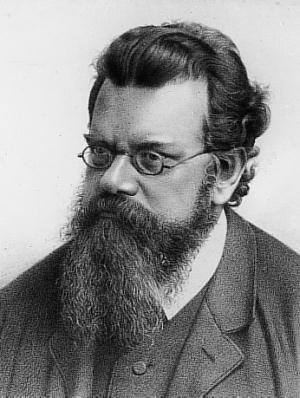
\includegraphics[width=\linewidth]{figures/boltzmann.jpeg}
      \caption{Ludwig Boltzmann~\cite{boltzmann}}
    \end{subfigure}%
    \quad
    \begin{subfigure}[b]{0.25\linewidth}
      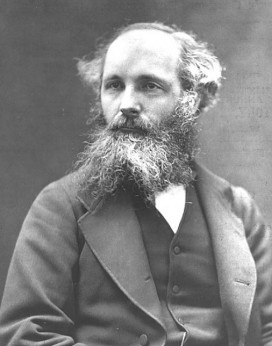
\includegraphics[width=\linewidth]{figures/maxwell.jpeg}
      \caption{James Clerk Maxwell~\cite{maxwell}}
    \end{subfigure}%
    \quad
    \begin{subfigure}[b]{0.25\linewidth}
      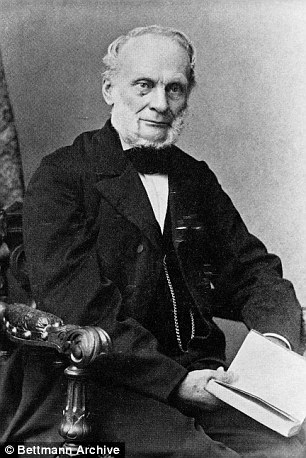
\includegraphics[width=\linewidth]{figures/clausius.jpeg}
      \caption{Rudolf Clausius~\cite{clausius}}
    \end{subfigure}
    \label{fig:the-greats}
  \end{figure}
\end{frame}

\begin{frame}{The Kinetic Theory of Gases}
  \begin{figure}[ht]
    \centering 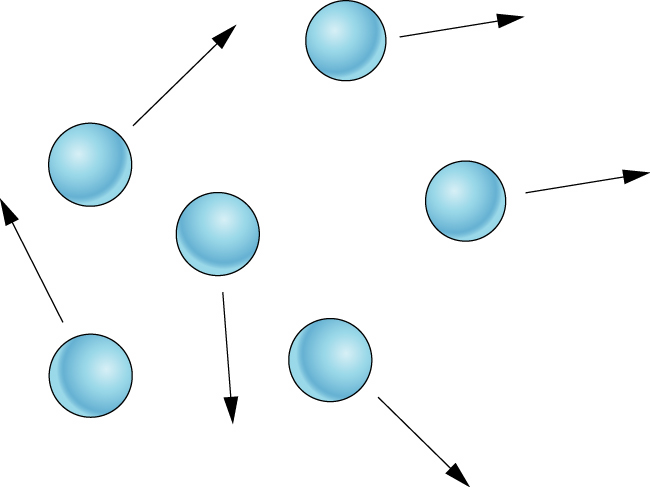
\includegraphics[width=0.5\linewidth]{figures/gas.jpg}
    \caption{Statistical physics began with the kinetic theory of
      gases, positing gases as collections of tiny
      particles\label{fig:label}.}
  \end{figure}
\end{frame}

\begin{frame}{The Fundamental Responsibility of Statistical Physicists}


  {\Huge Microscopic $\rightarrow$ Macroscopic}
\end{frame}

\begin{frame}{Ferromagnetism}
  \begin{figure}[ht]
    \centering
    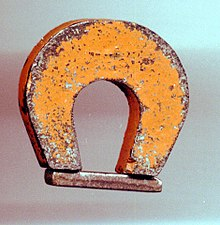
\includegraphics[width=0.5\linewidth]{figures/magnet.jpg}
    \caption{Ferromagnetism is the process by which materials like
      iron form permanent magnets~\cite{magnet}.}
  \end{figure}
\end{frame}

% Specifically, if we control the temperature and an external field,
% What will we MEASURE: - Magnetization, Susceptibility, Specific
% heat, etc.  We have to be a bit more precise with what we mean by
% MEASUREMENT MICROSTATE - how the atoms are configured and vibrating
% etc.  In square cm of air - million million million molecules No way
% to measure the microstate exactly (QM and Practical, data limits,
% etc) System is updating rapidly What we end up measure FUNDAMENTAL
% ASSUMPTION OF SM Clever reasaoning we can get to the boltzmann
% distribution For systems that exchange only energy to their
% surroundings, Probability is related to energy. More energy = less
% likely FUNDAMENTAL PROBLEM OF SM: Intractable Z. However Z also very
% useful.  PIVOT: Returning to our magnet, let's try an devise a suile
% energy model.  It turns out, the simplest we can do is the Ising
% model.

% PIVOT: To solve for probabilities and expectation vlaues we need
% energies
\begin{frame}{The Ising Model}
  \begin{figure}[ht]
    \centering
    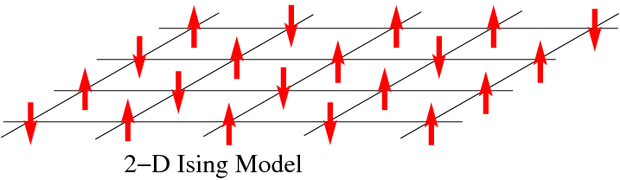
\includegraphics[width=0.75\textwidth]{figures/ising.png}
    \caption{The Ising model~\cite{ising}.\label{fig:ising} }
  \end{figure}
\end{frame}

\begin{frame}{Critical Phenomena and Phase Transitions}
  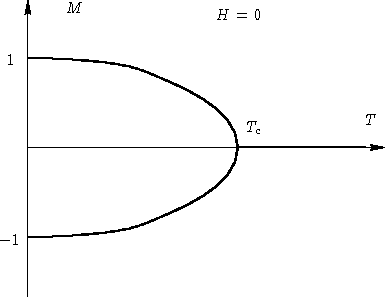
\includegraphics[width=.75\textwidth]{figures/correlation-length.png}
  \caption{The Ising model has a \textit{phase transition} between an ordered
    phase and a disordered phase.}
\end{frame}

\subsection{The Renormalization Group}
\begin{frame}{The Renormalization Group}
  \begin{figure}[ht]
    \centering
    
\includegraphics[width=.8\textwidth]{figures/block-rg.png}
    \caption{Three steps of majority-rule block-spin renormalization,
      preceding left to right (block size $b=2$).\label{fig:block-rg}}
  \end{figure}%

  {\large In RG, we reexpress our system in terms of a simpler set of
    variables, iterating to remove information about the
    shortest-distances.}

\end{frame}

% You can actually solve the Boltzmann distribution for this energy
% function in 1 and 2 dimensions 3 - proven to be NP-Hard PIVOT:
% Instead of solving these exactly, we'll consider approximate methods
% More representative of real-life investigations

\begin{frame}{Challenges in RG.}

  {\Large
  \begin{itemize}
  \item Devising RG procedure depends on system at hand.
  \item No obvious way to come up with appropriate transformations.
  \end{itemize}
  }
\end{frame}

\begin{frame}{Challenges in RG.}

  {\Large
  \begin{itemize}
  \item Devising RG procedure depends on system at hand.
  \item No obvious way to come up with appropriate transformations.
  \end{itemize}
  }

  {\Large Solution: Machine Learning}
\end{frame}

\section{Machine Learning}
\begin{frame}{Neural Networks}
  \begin{figure}[ht]
    \centering 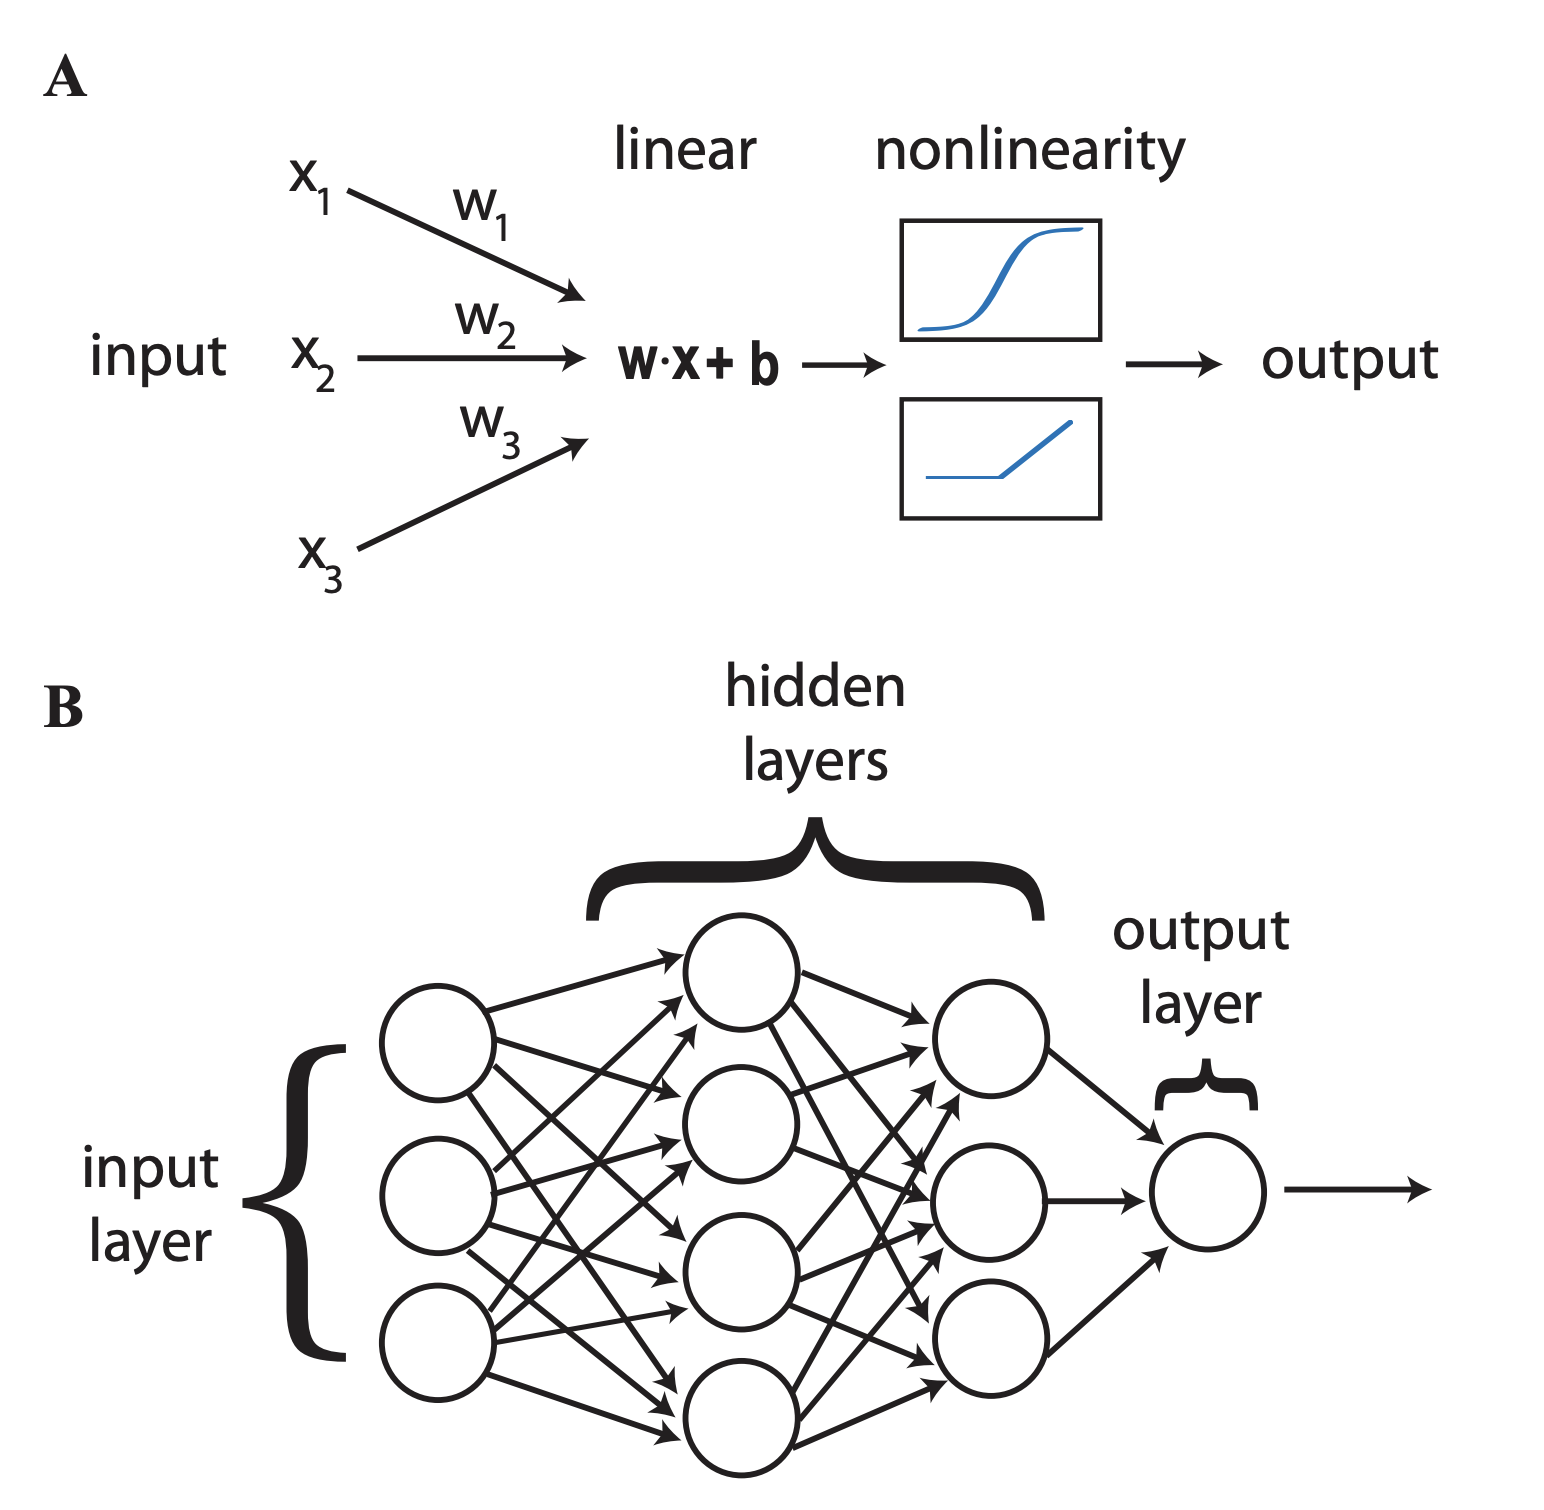
\includegraphics[width=0.7\linewidth]{figures/ffnn.png}
    \caption{A neural network consists of alternating linear and
      non-linear transformations~\cite{mehta-review}.}
  \end{figure}
\end{frame}

% Note qualitative similarities
\begin{frame}{Qualitative similarities between RG and RBMs}
  \begin{figure}[ht]
    \centering
    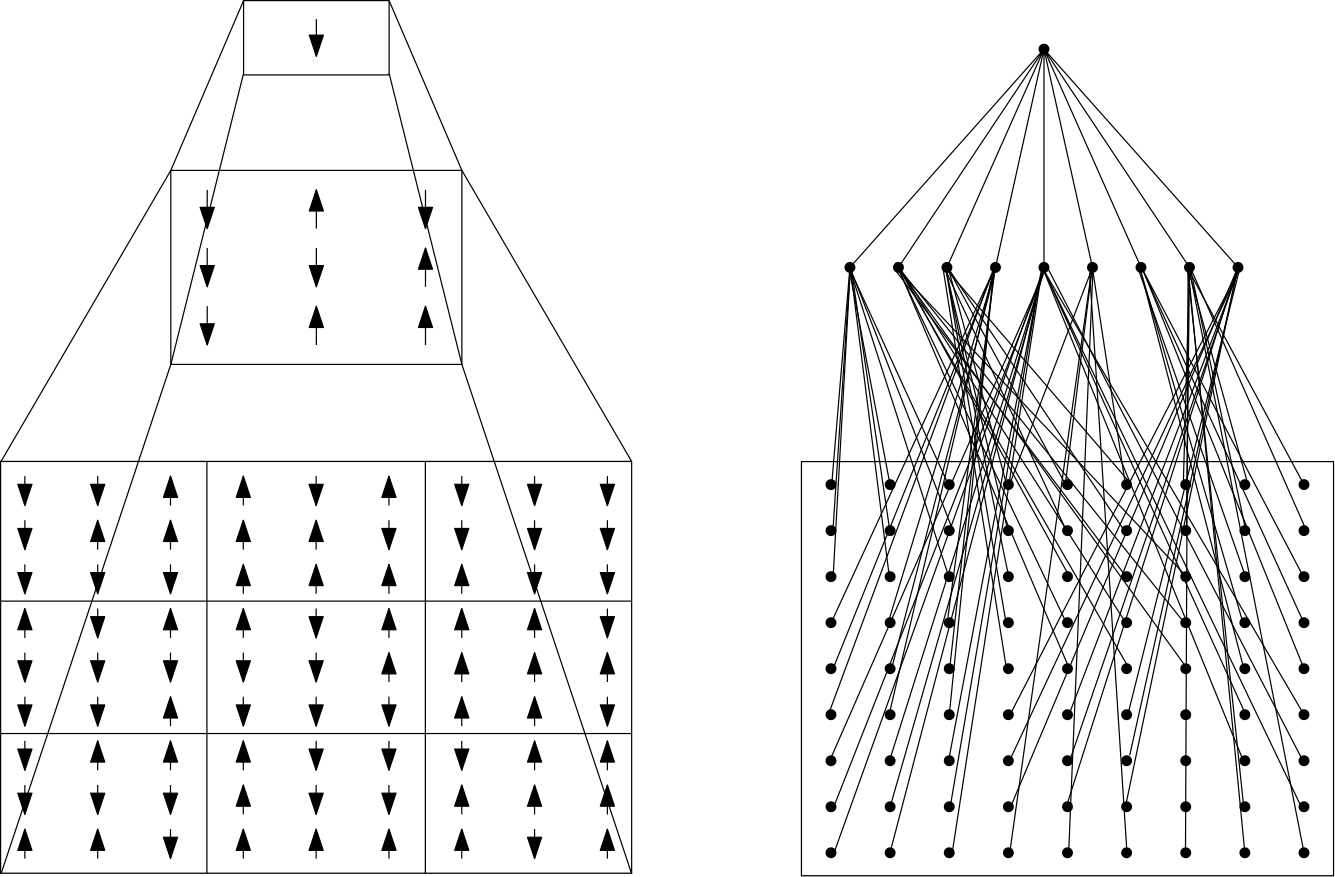
\includegraphics[width=0.5\textwidth]{figures/rg-rbm.png}
    \caption{Two iterations of block renormalization and a deep
      Boltzmann machine of three layers.\label{fig:rbm-rg} }
  \end{figure}
\end{frame}

\begin{frame}{Qualitative similarities between RG and RBMs}
  \begin{figure}[ht]
    \centering
    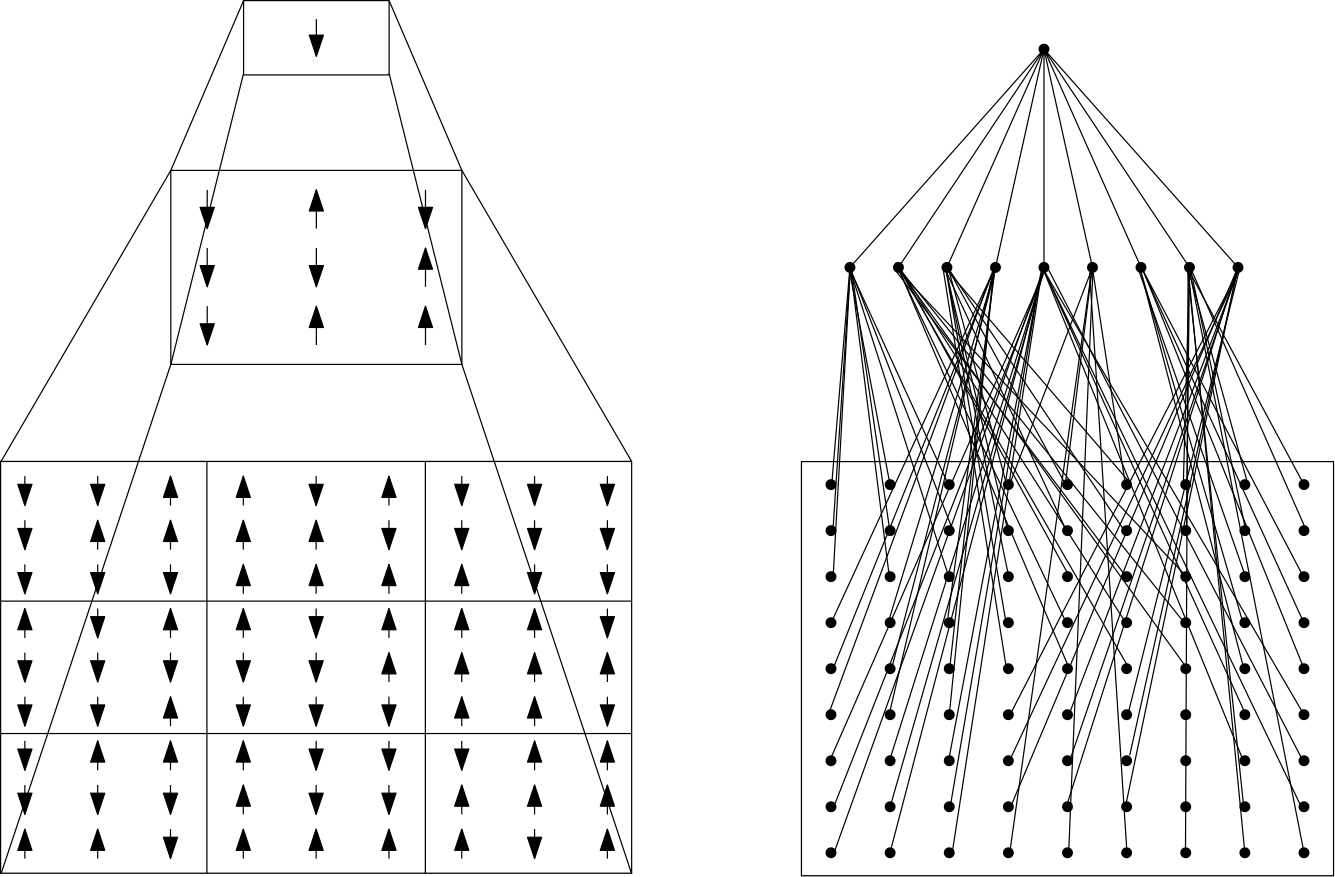
\includegraphics[width=0.5\textwidth]{figures/rg-rbm.png}
    \caption{Two iterations of block renormalization and a deep
      Boltzmann machine of three layers.\label{fig:rbm-rg} }
  \end{figure}
  {\Large Can we make this more precise?}
\end{frame}

\subsection{A Correspondence between Kadanoff's Variational RG and
  Generative RBMs}
\begin{frame}{An Exact Correspondence between Kadanoff's Variational
    RG and RBMs}

  \begin{figure}[ht]
    \centering
    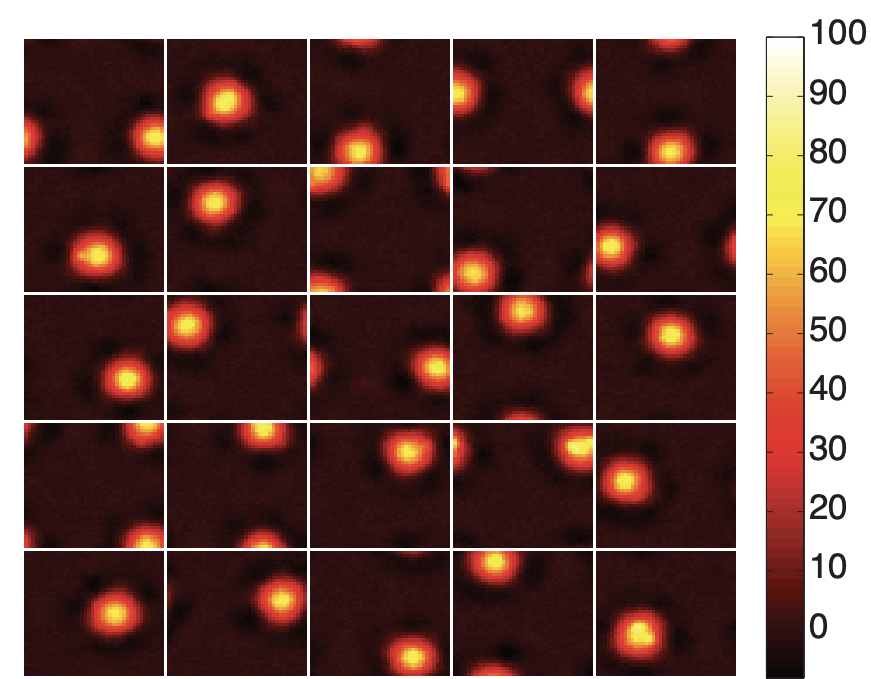
\includegraphics[width=0.5\textwidth]{figures/mehta.png}
    \caption{ The receptive fields of hidden units in
      DBMs~\cite{mehta}}.%
  \end{figure}%
  \begin{quote} Surprisingly, this local block spin structure emerges
    from the training process, suggesting the [deep neural network] is
    self-organizing to implement block spin
    renormalization~\cite{mehta}.
  \end{quote}
\end{frame}
%

\begin{frame}{Do RBMs Learn Block Spin RG?}

  {\huge General block spin tranformations are \textbf{NOT} all
    appropriate RG procedures.  }
\end{frame}

\begin{frame}{Extra conditions on RG Transformations}

  {\Large The Renormalization Group satisfies additional criteria that
    neural networks do not necessarily:}
  \begin{itemize}
  \item RG transformations (should) respect the symmetry of the system
    under investigation.
  \item RG transformations (should) extract only the long-distance
    information.
  \end{itemize}
\end{frame}

\begin{frame}{Information Theory}

  {\Large Information theory gives us an exact way to calculate:}
  \begin{itemize}
  \item The amount of information contained in a signal.
  \item The amount of \textit{relevant} information contained in a
    signal.
  \end{itemize}

\end{frame}

\begin{frame}{`rgpy' --- A python library for RG techniques.}
  \begin{figure}[ht]
    \centering 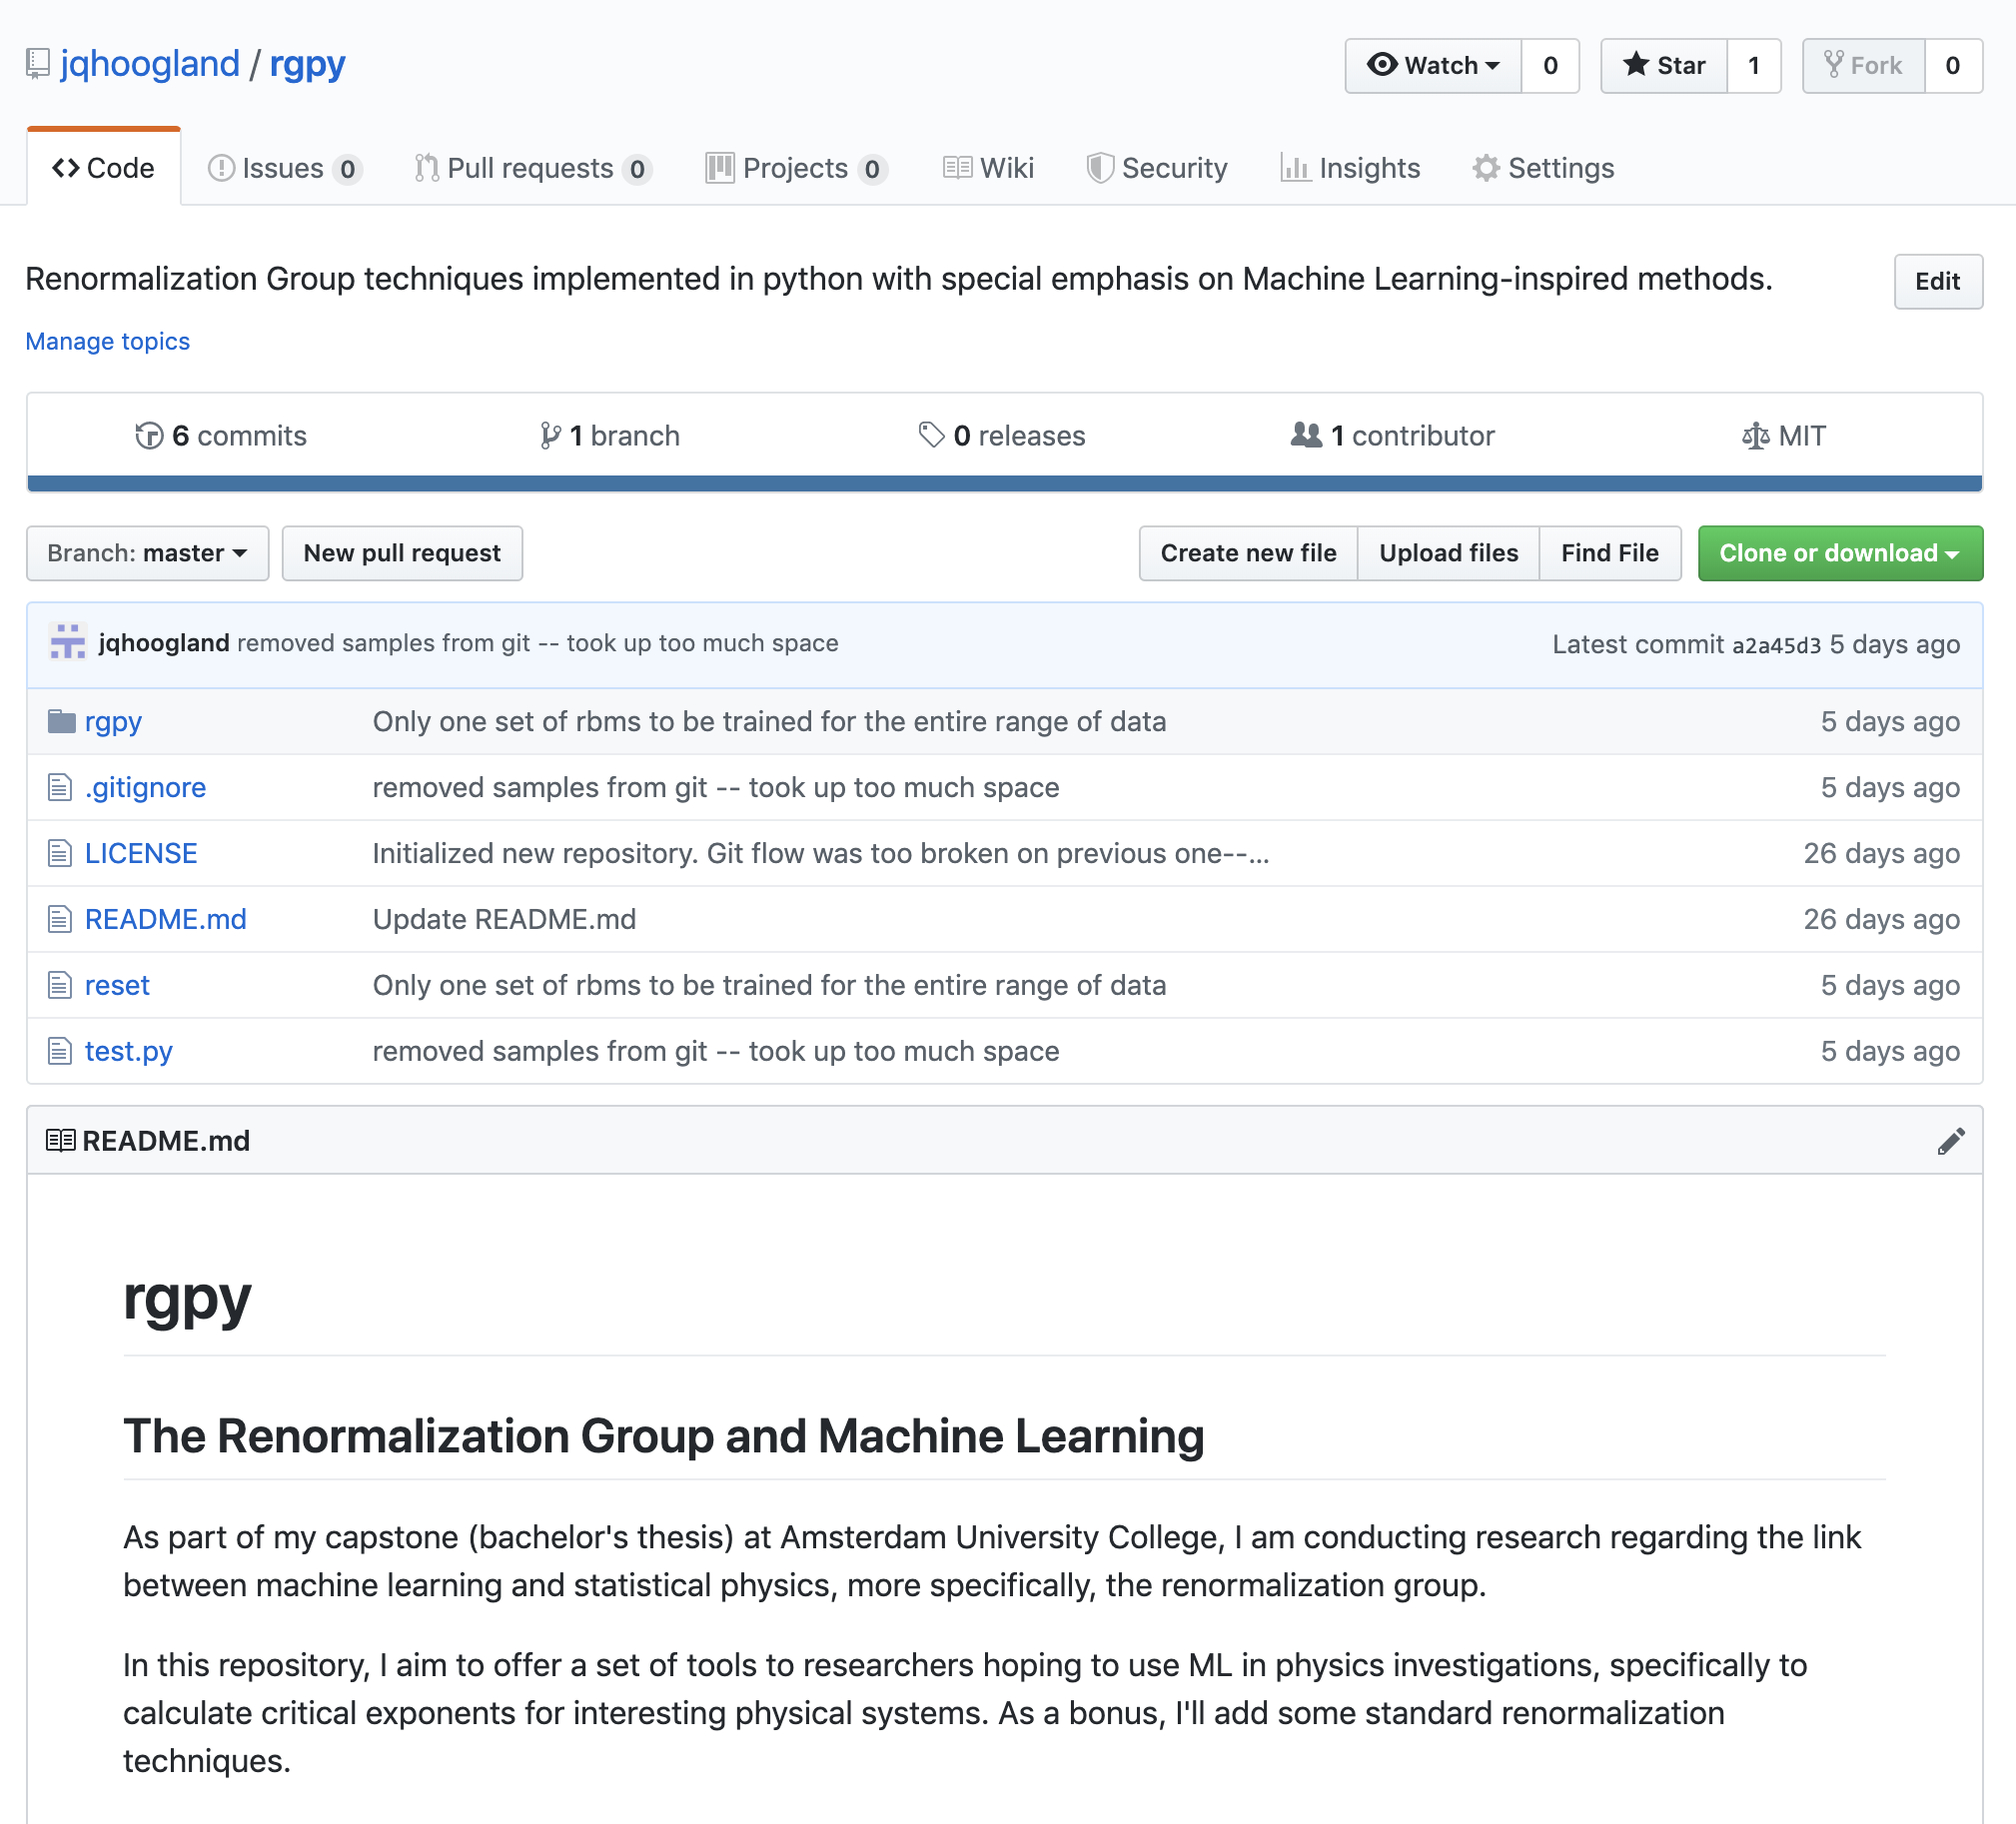
\includegraphics[width=0.8\textwidth]{figures/rgpy.png}
  \end{figure}

\end{frame}

\subsection{Calculating the Correlation-Length Critical Exponent}
\begin{frame}{A Recalculation of the Correlation-Length Critical Exponent}
  \begin{equation*}%
    \boxed{\nu\approx 0.79 \pm0.39}
  \end{equation*}%

  \begin{figure}
    \centering
    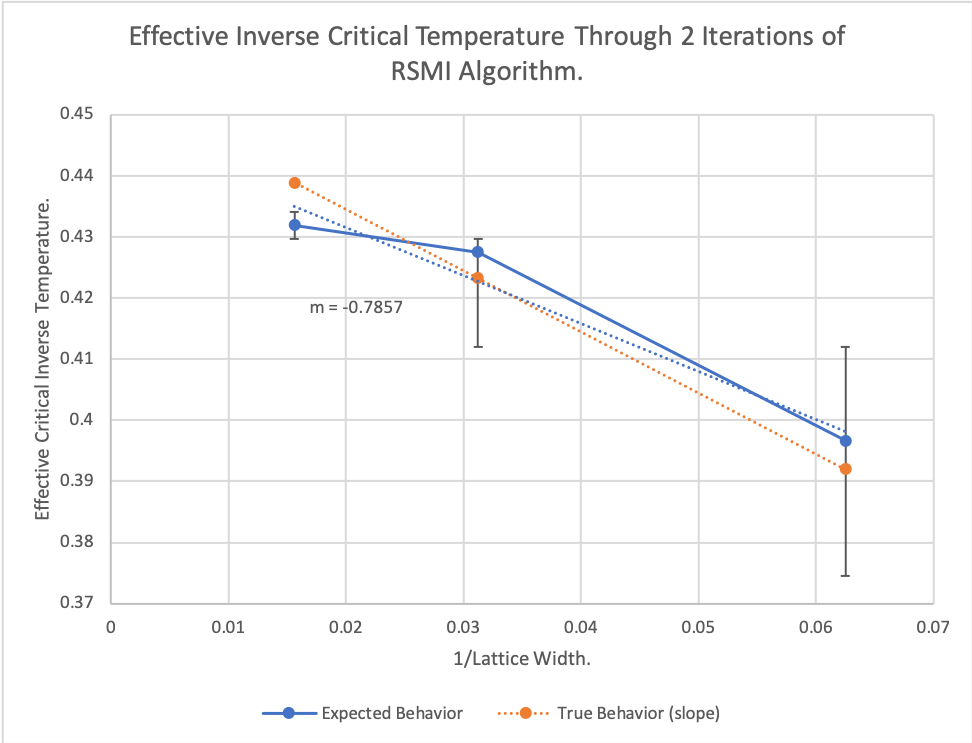
\includegraphics[width=0.5\textwidth]{figures/crit-exponent.png}
    \caption{Finite-size collapse curve for our implementation of the RSMI algorithm.}
  \end{figure}

\end{frame}
\subsection{Generalization}
\begin{frame}{Generalization to $n$-Spin and $O(n)$ Models}
  \begin{figure}[ht]
    \centering
    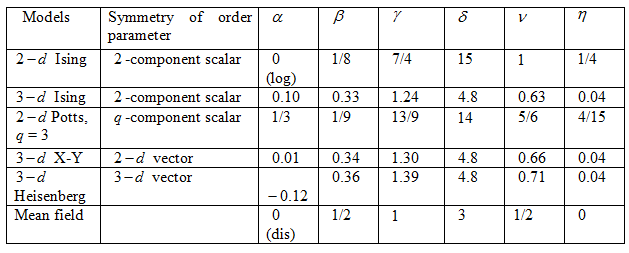
\includegraphics[width=0.9\textwidth]{figures/universality-classes.png}
    \caption{Universality classes for different numbers of dimensions
      $d$ and spin components $n$~\cite{universality-classes}.}
  \end{figure}
\end{frame}

% 1) this allowed us to
\section{Discussion and Conclusions}
\begin{frame}{Discussion and Conclusions}
  \begin{itemize}
  \item Information theory as conceptual framework for comparing ML
    and RG and devising \textit{optimal} procedures: e.g.\ the RSMI
    algorithm.
  \item Symmetries of our systems as restricting allowed RG and ML
    transformations and enabling understanding of ``black box'' neural
    networks: e.g.\ convolutional architectures.
  \item (Unsupervised) Machine learning as guiding the ``physical reasoning
    process,'' going beyond data analysis alone: e.g.\ calculating
    critical exponents~\cite{kjr}.
  \end{itemize}
\end{frame}


\section{References}
\begin{frame}{References}
  {\tiny

    \bibliographystyle{unsrt} \bibliography{references}
  }
\end{frame}

\end{document}
